\documentclass{article}
\usepackage[letterpaper, margin=1in, tmargin=0.5in, bmargin=0.7in]{geometry}
\usepackage{amsfonts}
\usepackage{graphicx}
\usepackage{amsmath}

\title{Ph 20 Assignment 3}
\author{Tawny Sit}
\date{October 29, 2017}

\begin{document}

\maketitle

\section{Simple Harmonic Oscillation (Mass on a Spring)}
For a mass on a spring, the equation of motion is:
$$  m\frac{d^2x}{dt^2} = -kx $$
The solution of the equation for the simple harmonic oscillator is of the form $x(t) = A\cos(\omega t) + B\sin(\omega t)$. Subsituting this solution into the equation, we find
$$ -m\omega^2(A\cos(\omega t) + B\sin(\omega t)) = -k(A\cos(\omega t) + B\sin(\omega t)) $$
$$ m\omega^2 = k $$
$$ \omega = \sqrt{\frac{k}{m}}$$
We also see that at $t=0$, $x(0) = A$ and $x'(0) = \omega B$. Thus, the general solution to a mass on a spring is
$$ x(t) = x(0)\cos(\omega t) + \frac{1}{\omega}x'(0)\sin(\omega t) $$
where $\omega = \sqrt{\frac{k}{m}}$. Therefore, we see that
$$v(t) = x'(t) = -x(0)\omega\sin(\omega t) + x'(0)\cos(\omega t)$$
We use this solution with $ \omega = 1 $ as the analytic solution in our Python program. The following is the plot of $x(t)$ and $v(t)$ as a function of time, with $ x(0) = 1 $ and $ v(0) = 0 $:

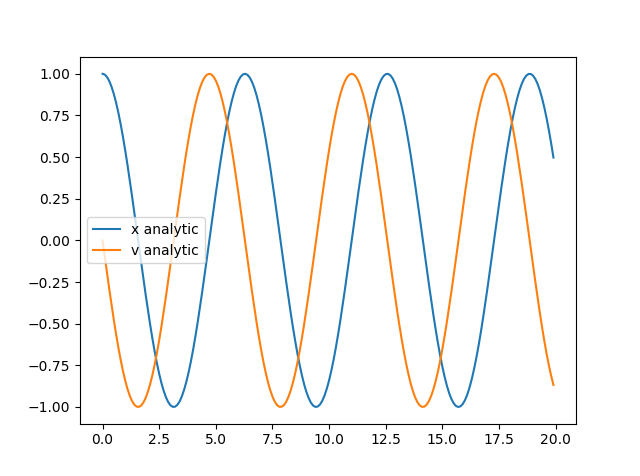
\includegraphics[scale=0.9]{analytic_solution.jpg}

\section{The Explicit Euler Method}

\subsection{Numerical Integration}
Implementing the explicit Euler method in Python was simple and straightforward given the equations for $x_{i+1}$ and $v_{i+1}$. The following graph was produced with the same conditions as the graph of the analytic solution, namely $ x(0) = 1 $ and $ v(0) = 0 $. The step size was set to $ h = 0.1 $ which was small enough to produce a smooth graph and large enough to show visible errors within a few oscillations.

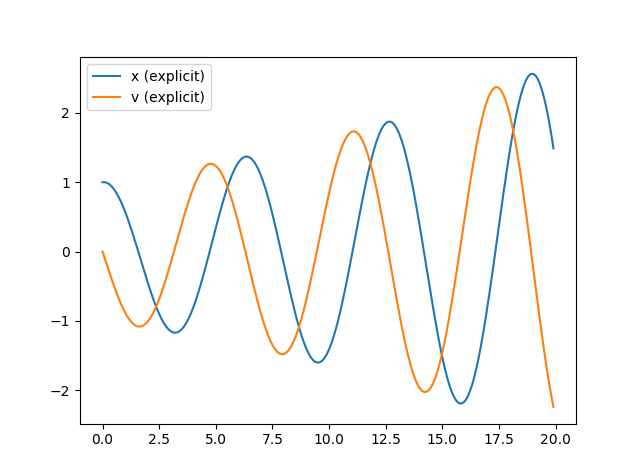
\includegraphics[scale=0.9]{explicit_solution.jpg}

For comparison, a plot of the analytic solution and the numerical integration:

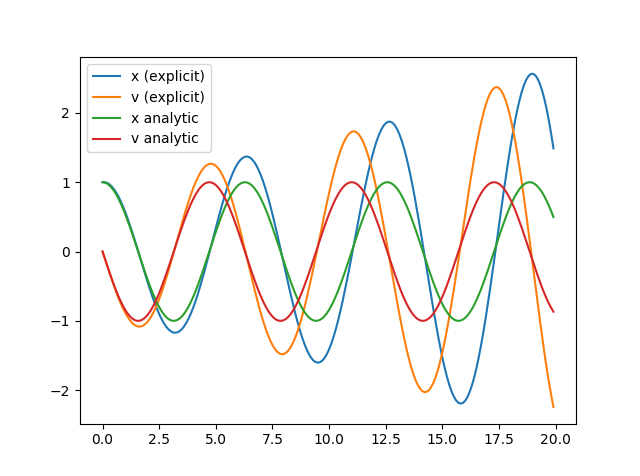
\includegraphics[scale=0.9]{analytic_vs_explicit.jpg}

\subsection{Global Errors}
The global error was computed for each time step using $ x_{analytic}(t_i) - x(t_i) $ and $ v_{analytic}(t_i) - v(t_i) $.

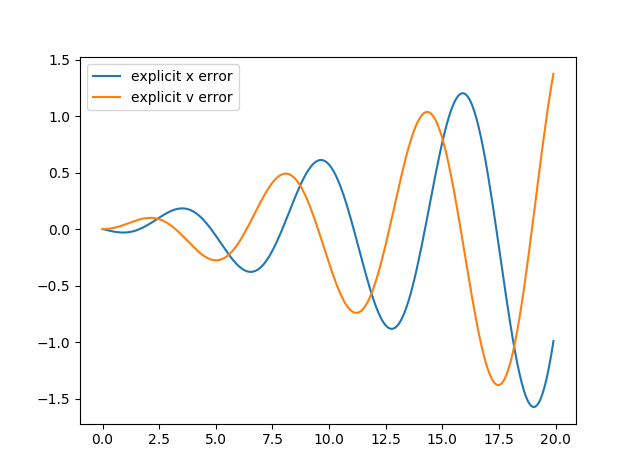
\includegraphics[scale=0.9]{explicit_error.jpg}

The absolute magnitude of the error clearly increases with time.

\subsection{Truncation Error}
The truncation error was calculated to be the maximum global error for a certain time step size. The step sizes used were $h_0, \frac{h_0}{2}, \frac{h_0}{4}, \frac{h_0}{8}, \frac{h_0}{16}$ with $h_0 = 0.1$.

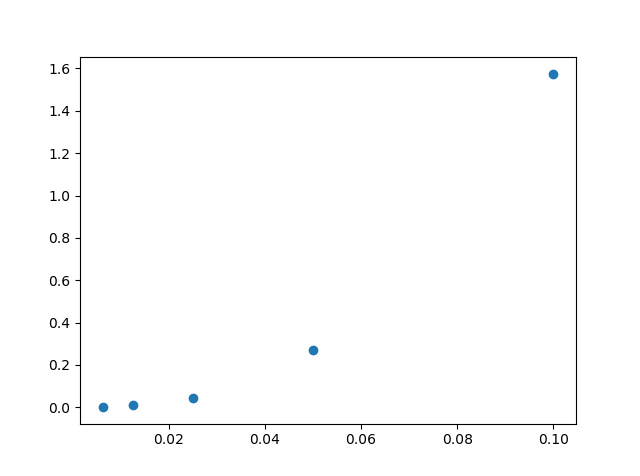
\includegraphics[scale=0.9]{truncation_error.jpg}

The error clearly grows with step size, but it appears more exponential than simply linearly proportional as suggested in the assignment.

\subsection{Evolution of Total Energy}
The normalized energy $E = x^2 + v^2 $ was calculated with the $x$ and $v$ values from numerical integration.

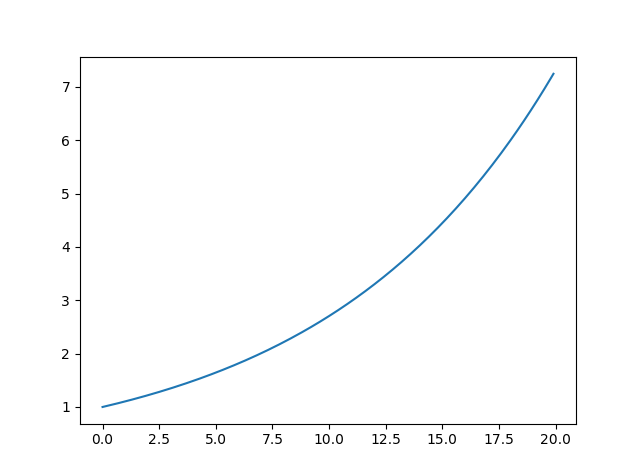
\includegraphics[scale=0.9]{explicit_energy.jpg}

We know that the energy in a simple harmonic oscillator should be conserved, but the numerical integration clearly shows that the energy in the system grows exponentially. The growth of the energy in the system increases with time with the error in the numerical integration.

\section{The Implicit Euler Method}

\subsection{Finding the Equations for Numerical Integration}
From the assignment, we need to solve the system
\[
\begin{pmatrix}
    1 & -h \\
    h & 1
\end{pmatrix}
\begin{pmatrix}
    x_{i+1} \\
    v_{i+1}
\end{pmatrix}
=
\begin{pmatrix}
    x_i \\
    v_i
\end{pmatrix}
\]
to get function of $x_{i+1}$ and $v_{i+1}$. This is done simply by multiplying by the inverse matrix of
$\begin{pmatrix}
    1 & -h \\
    h & 1
\end{pmatrix}$ as follows:
\[
\frac{1}{h^2 + 1}
\begin{pmatrix}
    1 & h \\
    -h & 1
\end{pmatrix}
\begin{pmatrix}
    1 & -h \\
    h & 1
\end{pmatrix}
\begin{pmatrix}
    x_{i+1} \\
    v_{i+1}
\end{pmatrix}
=
\frac{1}{h^2 + 1}
\begin{pmatrix}
    1 & h \\
    -h & 1
\end{pmatrix}
\begin{pmatrix}
    x_i \\
    v_i
\end{pmatrix}
\]
\[
\begin{pmatrix}
    x_{i+1} \\
    v_{i+1}
\end{pmatrix}
=
\frac{1}{h^2 + 1}
\begin{pmatrix}
    x_i + hv_i \\
    -hx_i + v_i
\end{pmatrix}
\]
Thus we find that, using the implicit Euler method for the mass on a spring,
$$ x_{i+1} = \frac{x_i + hv_i}{h^2 + 1} $$
$$ v_{i+1} = \frac{v_i - hx_i}{h^2 + 1} $$

\subsection{Numerical Integration}
Once the formulas for $ x_{i+1} $ and $ v_{i+1} $ were found as seen above, implementing the implicit Euler method was the same as with the explicit Euler method, just with different formulas for $ x_{i+1} $ and $ v_{i+1} $. The following graph was produced with the same conditions as the explicit integration, $ x(0) = 1 $, $ v(0) = 1 $, and $ h = 0.1 $.

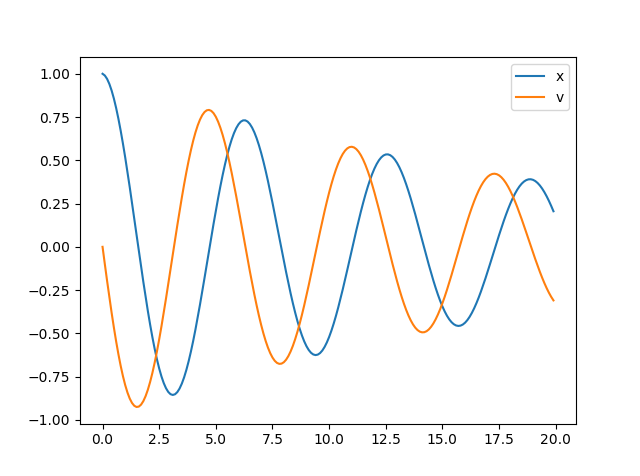
\includegraphics[scale=0.9]{implicit_solution.jpg}

For easier comparison, a plot of the analytic solution and the implicit integration:

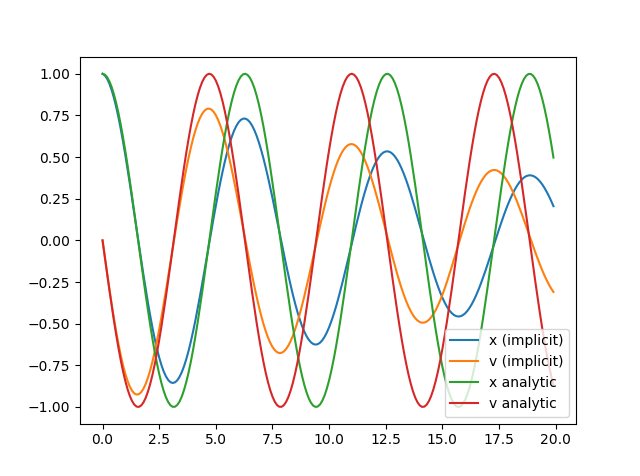
\includegraphics[scale=0.9]{analytic_vs_implicit.jpg}

Unlike the explicit case, the error using the implicit method seems to come from the values decreasing rather than increasing. For more direct comparison, the explicit and implicit method results on the same graph:

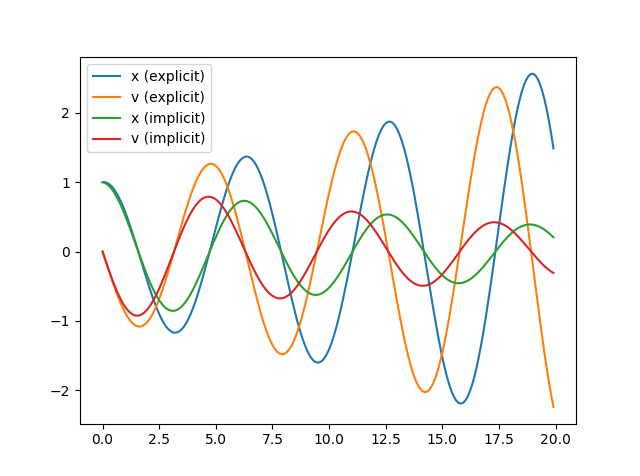
\includegraphics[scale=0.9]{implicit_vs_explicit.jpg}

\subsection{Global Errors}
The same process as the explicit method was used to calculate global error for the implicit method.

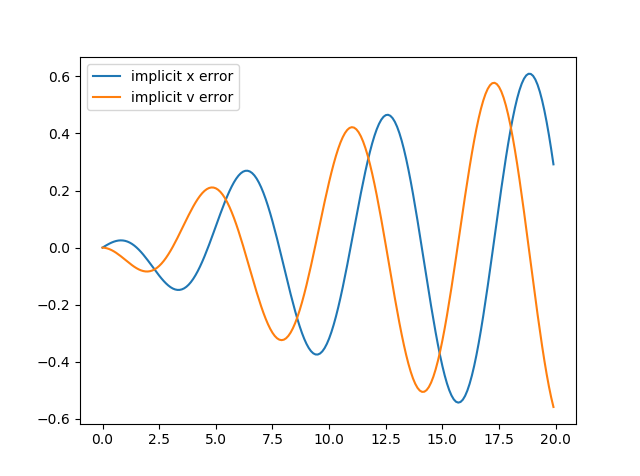
\includegraphics[scale=0.9]{implicit_error.jpg}

Despite the opposite trend in actual values, the implicit method still produces increasing error over time. However, the following plot of implicit vs. explicit error shows that despite the increase, the implicit method's error increases more slowly compared to the explicit method:

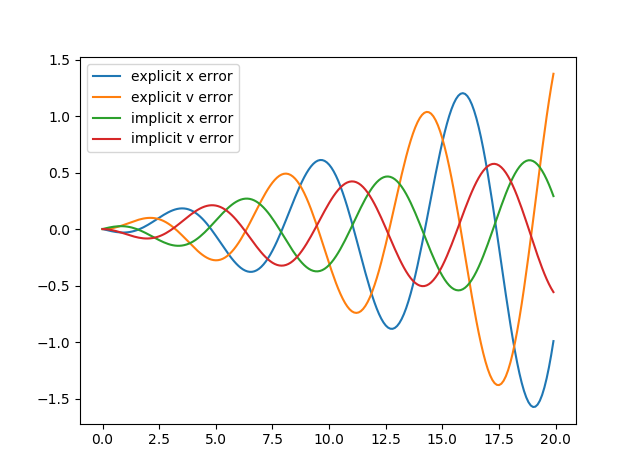
\includegraphics[scale=0.9]{implicit_vs_explicit_error.jpg}

Additionally, it is interesting to note that the times of positive and negative error values are switched for the implict and explicit integrations.

\subsection{Evolution of Total Energy}
The same process as the explicit method was used to calculate global error for the implicit method.

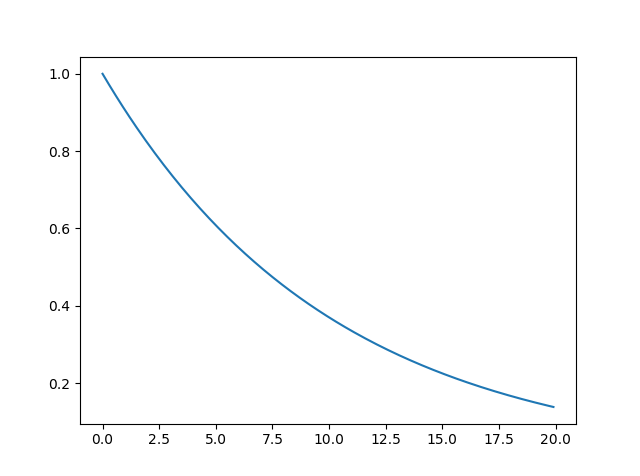
\includegraphics[scale=0.9]{implicit_energy.jpg}

Unlike the explicit case, energy decreases over time for the implicit integration. However, this is still not we would expect from a simple harmonic oscillator which conserves energy.

\section{Phase Space Geometry}
\subsection{The Explicit and Implicit Euler Methods}
It is known that the phase space plot, $x$ vs. $v$, should be a closed circle (or oval, if the physical scale of each side of the plot is different). To check, the following is a plot of just the analytic solution's phase space geometry:

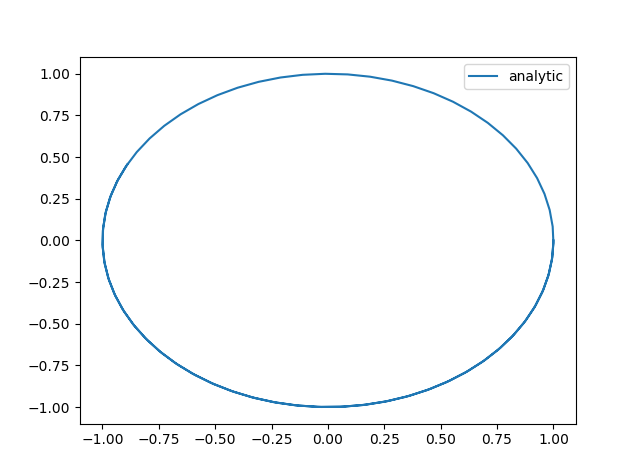
\includegraphics[scale=0.9]{analytic_phasespace.jpg}

This is exactly what we expect. Next, we plot the explicit and implicit phase space geometries with the analytic geometry for comparison:

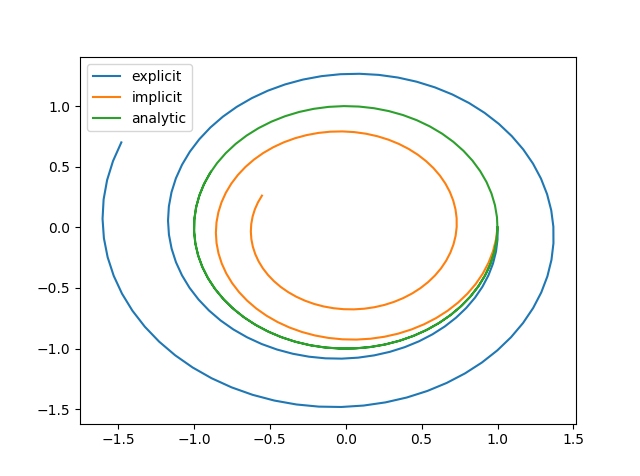
\includegraphics[scale=0.9]{implicit_vs_explicit_vs_analytic_phasespace.jpg}

It is very clear that the explicit and implicit solutions do not form closed circles; rather, they form spiral shapes. For this plot, the total time of integration was set to 10 rather than the previous 20 so as not to clutter the plot too much, but the step size was still $ h = 0.1 $.

\subsection{The Sympletic Euler Method}
The sympletic Euler method was coded the same way as the explicit and implicit methods with the notable constraint that due to the dependence on $ x_{i+1} $ of $ v_{i+1} $, the value of $ v_{i+1} $ \textit{had} to be calculated \textit{after} $ x_{i+1} $ was calculated. For the previous methods, the order did not matter; it was an arbitary choice to calculate $ x_{i+1} $ before $ v_{i+1} $. For the same $ h = 0.1 $, the phase space plot using the sympletic Euler method is

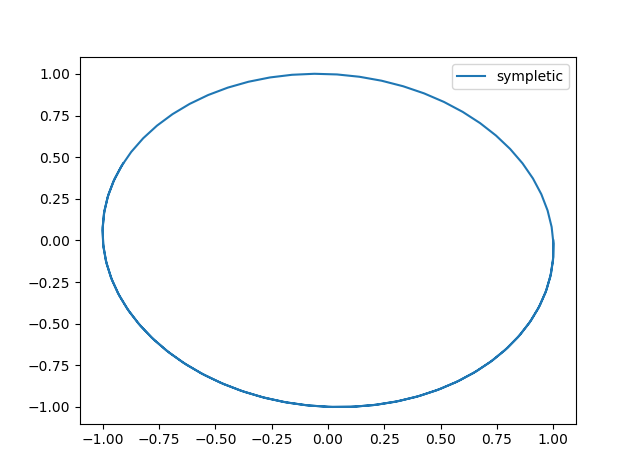
\includegraphics[scale=0.9]{sympletic_phasespace.jpg}

This is only slightly different (but still different!) than the phase space plot of the analytic solution, as shown:

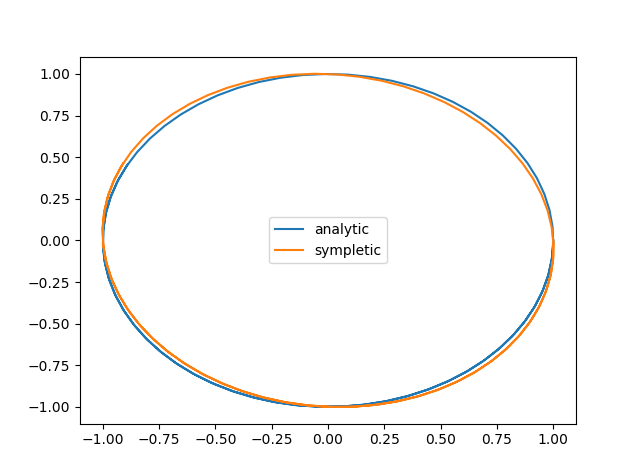
\includegraphics[scale=0.9]{analytic_vs_sympletic_phasespace.jpg}
\subsection{Energy of the Sympletic Euler Method}
The plot of the energy (still defined $ E = x^2 + v^2 $) of the sympletic Euler method vs. the analytic energy speaks for itself. The step size used was still $ h = 0.1 $.

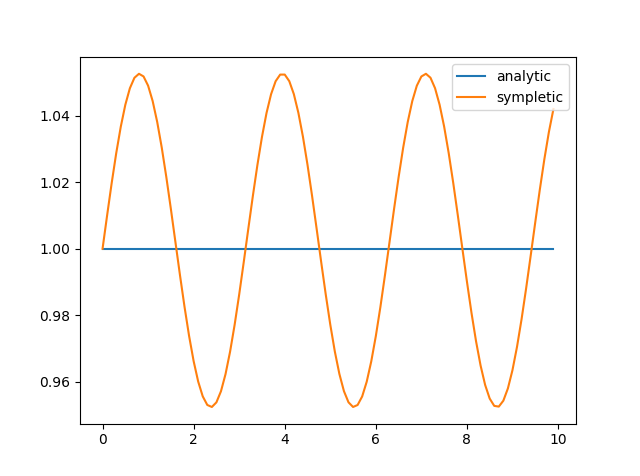
\includegraphics[scale=0.9]{analytic_vs_sympletic_energy.jpg}

The energy from the sympletic integration is sinusoidal; it should average to the appropriate constant value over time but is not at that value over small time intervals. This is reflective of what was seen in the analytic vs. sympletic phase space diagram where the sympletic geometry was also a closed loop but it was tilted such that certain parts of the sympletic trajectory were inside the analytic circle and other parts outside. These likely correspond to the sinusoidal nature of the sympletic energy.

\section{Notes on Python Files}
\texttt{euler.py} is the code from Part 1 of the assignment. \texttt{phasespace.py} is the code from Part 2 of the assignment. Changes in initial values such as $ x(0), v(0), h $ are made directly in the code, and control of which plots are produced is based on commenting in/out \texttt{plt.plot()} lines.

\end{document}
